\documentclass[11pt]{article}
\usepackage[margin=1in]{geometry}
\usepackage{amsmath,amssymb,bm}
\usepackage{booktabs,array,longtable}
\usepackage{graphicx}
\usepackage{hyperref}
\usepackage{enumitem}
\graphicspath{{../figures/}{figures/}}

\newcommand{\R}{\mathbb{R}}
\newcommand{\one}{\mathbf{1}}
\newcommand{\w}{\bm{w}}
\newcommand{\bmu}{\bm{\mu}}

\title{DS5020 Final Project -- Iteration 3\\[2pt]
\large Portfolio Optimization: Small Worked Example and Verification}
\author{Vinh Pham \and Tung Nguyen}
\date{Fall 2026}

\begin{document}
\maketitle

\section*{Task Assignment}
\begin{tabular}{@{}llll@{}}
\toprule
ID & Task & Owner & Checker\\
\midrule
E1 & Small worked example (step by step) & Vinh Pham & Tung Nguyen\\
S5 & Simulation test: recover the known truth & Tung Nguyen & Vinh Pham\\
S6 & Run on the real data and verify & Vinh Pham & Tung Nguyen\\
A2 & Check assumptions on the data & Vinh Pham & Tung Nguyen\\
M1 & Iteration 3 math questions & Vinh Pham & Tung Nguyen\\
\bottomrule
\end{tabular}

\section{Small Worked Example: Two-Asset Minimum Variance}\label{sec:small-example}
The calculations are implemented with exact fractions in
\texttt{src/small\_example.py}. Let
\[
R=\begin{bmatrix}0&0\\0&1/5\\1/5&1/5\\1/5&1/5\end{bmatrix},
\qquad T=4,\quad N=2,\qquad
\one_T=\begin{bmatrix}1\\1\\1\\1\end{bmatrix},\quad
\one=\begin{bmatrix}1\\1\end{bmatrix}.
\]

\textbf{Step (1): Sample mean.}
We average each asset's returns:
\[
R^\top\one_T=\begin{bmatrix}2/5\\3/5\end{bmatrix},
\qquad
\hat\bmu=\frac14 R^\top\one_T=
\begin{bmatrix}1/10\\3/20\end{bmatrix}.
\]

\textbf{Step (2): Center the data.}
Subtract the corresponding sample mean from each column:
\[
\one_T\hat\bmu^\top=
\begin{bmatrix}1/10&3/20\\1/10&3/20\\1/10&3/20\\1/10&3/20\end{bmatrix},
\qquad
R_c=R-\one_T\hat\bmu^\top=
\begin{bmatrix}-1/10&-3/20\\-1/10&1/20\\1/10&1/20\\1/10&1/20\end{bmatrix}.
\]

\textbf{Step (3): Sample covariance.}
\[
R_c^\top R_c=\begin{bmatrix}1/25&1/50\\1/50&3/100\end{bmatrix},
\qquad
\hat\Sigma=\frac1{T-1}R_c^\top R_c
=\begin{bmatrix}1/75&1/150\\1/150&1/100\end{bmatrix}.
\]
The leading principal minor is $1/75>0$ and
$\det(\hat\Sigma)=1/11250>0$, so $\hat\Sigma$ is positive definite.

\textbf{Step (4): Gaussian elimination.}
Following the Iteration 2 minimum-variance and target-return derivations, solve
$\hat\Sigma\bm x=\one$ and $\hat\Sigma\bm y=\hat\bmu$ together.
The first pivot is $1/75$; applying $R_2\leftarrow R_2-\frac12 R_1$ gives
\[
\left[\begin{array}{cc|cc}
1/75&1/150&1&1/10\\
1/150&1/100&1&3/20
\end{array}\right]\longrightarrow
\left[\begin{array}{cc|cc}
1/75&1/150&1&1/10\\
0&1/150&1/2&1/10
\end{array}\right].
\]
Back substitution yields
\[
x_2=75,\quad x_1=\frac{1-(1/150)x_2}{1/75}=\frac{75}{2},
\qquad
y_2=15,\quad y_1=\frac{1/10-(1/150)y_2}{1/75}=0.
\]
Thus $\bm x=(75/2,75)^\top$ and $\bm y=(0,15)^\top$.
Multiplication verifies $\hat\Sigma\bm x=\one$ and
$\hat\Sigma\bm y=\hat\bmu$.

\textbf{Step (5): Frontier constants.}
Target-return derivation,
\[
\begin{aligned}
a&=\one^\top\bm x=75/2+75=225/2,\\
b&=\hat\bmu^\top\bm x=(1/10)(75/2)+(3/20)(75)=15,\\
c&=\hat\bmu^\top\bm y=(1/10)(0)+(3/20)(15)=9/4,\\
d&=ac-b^2=(225/2)(9/4)-15^2=225/8>0.
\end{aligned}
\]

\textbf{Step (6): Global minimum-variance portfolio.}
Minimum-variance formula,
\[
\w^*=\frac{\bm x}{a}
=\frac{\begin{bmatrix}75/2\\75\end{bmatrix}}{225/2}
=\begin{bmatrix}1/3\\2/3\end{bmatrix}.
\]
Portfolio return and risk result, the expected return is
$\hat\bmu^\top\w^* = 2/15$ and the variance is
\[
\hat\Sigma\w^*=\begin{bmatrix}2/225\\2/225\end{bmatrix},
\qquad
\w^{*\top}\hat\Sigma\w^*=2/225=1/a.
\]

\textbf{Step (7): Target-return portfolio.}
For $r=1/5$, the Iteration 2 target-return derivation gives the augmented multiplier system.
Partial pivoting swaps the two rows:
\[
\left[\begin{array}{cc|c}9/4&15&1/5\\15&225/2&1\end{array}\right]
\longrightarrow
\left[\begin{array}{cc|c}15&225/2&1\\9/4&15&1/5\end{array}\right].
\]
Then $R_2\leftarrow R_2-\frac3{20}R_1$ gives
\[
\left[\begin{array}{cc|c}15&225/2&1\\0&-15/8&1/20\end{array}\right].
\]
Back substitution gives $\lambda_2=-2/75$ and $\lambda_1=4/15$.
\[
\w(r)=\lambda_1\bm y+\lambda_2\bm x
=\begin{bmatrix}0\\4\end{bmatrix}+\begin{bmatrix}-1\\-2\end{bmatrix}
=\begin{bmatrix}-1\\2\end{bmatrix}.
\]
The negative weight represents short selling.
Direct substitution confirms the budget and target-return constraints:
\[
\one^\top\w(r)=1,\qquad \hat\bmu^\top\w(r)=1/5.
\]
By the Iteration 2 efficient-frontier formula, the direct variance agrees with the frontier formula:
\[
\w(r)^\top\hat\Sigma\w(r)=2/75
=\lambda_1 r+\lambda_2=\frac{ar^2-2br+c}{d}.
\]
Also, $\hat\Sigma\w(r)=(0,1/75)^\top
=\lambda_1\hat\bmu+\lambda_2\one$.

\textbf{Second-way verification.}
The budget constraint gives $\one^\top\w^*=1/3+2/3=1$.
With $\lambda=2/a=4/225$, the exact Lagrangian stationarity residual is
\[
2\hat\Sigma\w^*-\lambda\one=
2\begin{bmatrix}2/225\\2/225\end{bmatrix}
-\frac4{225}\begin{bmatrix}1\\1\end{bmatrix}
=\begin{bmatrix}0\\0\end{bmatrix}.
\]
Independently, writing $w_2=1-w_1$ and differentiating the resulting
scalar quadratic gives
\[
w_1=\frac{\hat\Sigma_{22}-\hat\Sigma_{12}}
{\hat\Sigma_{11}+\hat\Sigma_{22}-2\hat\Sigma_{12}}=\frac13,\qquad
w_2=\frac23.
\]
The exact weight difference is zero.

\section{Simulation Test: Recover the Known Truth}
\textbf{Model.} $\bm r_t \overset{\text{iid}}{\sim}\mathcal N(\bmu,\Sigma)$, $N=4$, $T=2000$, seed \texttt{default\_rng(0)}, with
$\bmu=(0.05,0.08,0.12,0.07)^\top$, volatilities $(0.10,0.15,0.25,0.12)$, and $\Sigma = \operatorname{diag}(\text{vol})\,C\,\operatorname{diag}(\text{vol})$ for the correlation matrix
\[
C=\begin{bmatrix}
1&0.3&0.2&0.1\\
0.3&1&0.4&0.2\\
0.2&0.4&1&0.3\\
0.1&0.2&0.3&1
\end{bmatrix}.
\]
The true minimum-variance weights are computed from this known $\Sigma$,
independently of the sampled returns.

The script \texttt{src/check\_simulation.py} uses the same model and main
seed as Iteration 2. The core method uses NumPy arrays and matrix operations; \texttt{numpy.linalg} is used only for independent references and diagnostics.

\subsection{Truth and library comparisons}
At $T=2000$ (seed 0), the true weights are
$(0.5296,0.1277,-0.0275,0.3701)^\top$ and the estimated weights are
$(0.5316,0.1406,-0.0338,0.3616)^\top$.
The Euclidean error is $0.0168$; the largest component error is $0.0128$.
The sample mean errors in standard-error units are
$(-0.44,-0.21,-0.40,-0.74)$, all within three standard errors.
The standard error of $\hat\mu_i$ is $\sqrt{\Sigma_{ii}/T}$.

\subsection{Error against sample size}
We run 200 independent replications at each sample size, with seeds
1000--1199. The main comparison still uses seed 0. For each sample
size, the component standard errors are the empirical standard deviations
of the replicated weights, and the RMSE is
$\sqrt{\frac1{200}\sum_{j=1}^{200}\|\hat\w_j-\w^*\|_2^2}$.
\begin{center}
\begin{tabular}{rrrrr}
\toprule
$T$ & Seed-0 error & RMSE over replications & Max. error / SE & Within 3 SE?\\
\midrule
50 & 0.0240 & 0.1619 & 0.19 & Yes\\
500 & 0.0372 & 0.0497 & 1.16 & Yes\\
2000 & 0.0168 & 0.0234 & 1.00 & Yes\\
5000 & 0.0071 & 0.0151 & 0.65 & Yes\\
\bottomrule
\end{tabular}
\end{center}
The single-run error need not decrease monotonically. The fitted log--log
slope of the replicated RMSE is $-0.518$, close to the expected $-1/2$.

\begin{figure}[htbp]\centering
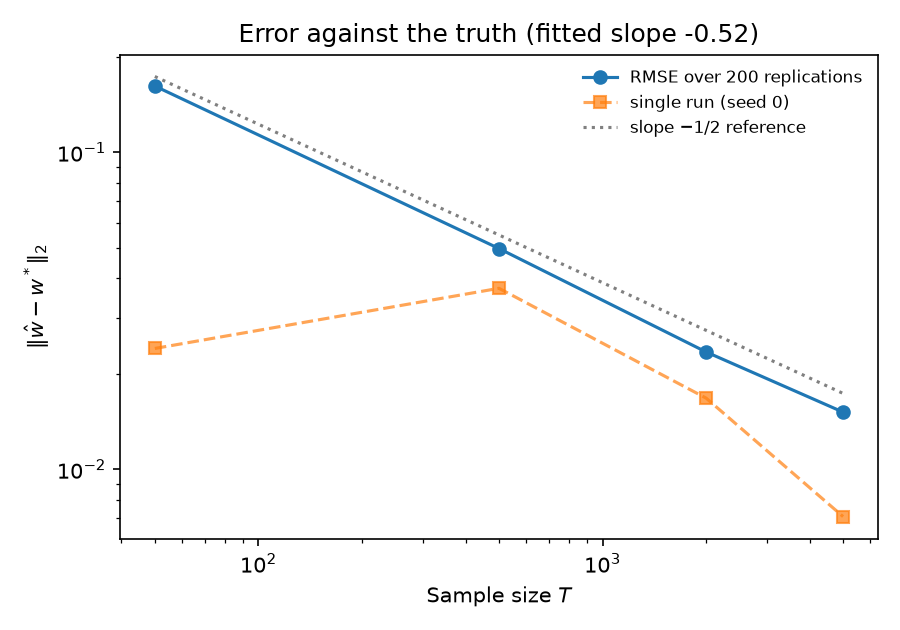
\includegraphics[width=0.72\linewidth]{sim_error_vs_T.png}
\caption{Weight error against sample size; replicated RMSE and seed-0 error.}
\end{figure}

\subsection{Stress tests}
The short sample with $T=60$ uses seed 1 as in Iteration 2. Its weight error
is $0.1530$, about 9.1 times the main-run error of $0.0168$.
The condition number increases from $8.06$ to $10.62$.

For a deliberate violation of positive definiteness, append a fifth asset
identical to the first. Then $R_c(\bm e_1-\bm e_5)=0$, so
$\hat\Sigma(\bm e_1-\bm e_5)=0$. The smallest computed eigenvalue is
$-2.61\times10^{-18}$ (zero in exact arithmetic), and the condition
number is $1.14\times10^{17}$. Splitting the first asset's weight between
the two identical assets does not change the portfolio variance:
both tested portfolios have variance $0.0064118817$.
The minimizer is not unique, and division by a near-zero pivot in floating
point produces unreliable weights. The inverse formula requires positive
definiteness.


\section{Run on the Real Data and Verify}
\textbf{Source.} Adjusted closing prices from Yahoo Finance
(\texttt{yfinance}) for AAPL, NVDA, GOOGL, META, AMZN, AMD, PLTR, MU,
and INTC, using the same dates as Iteration 2. SpaceX was excluded
in Iteration 2 because its trading history would shorten the common window.

\subsection{Library comparison}
We independently estimate $\hat\bmu$ with NumPy's mean and
$\hat\Sigma$ with \texttt{numpy.cov} using divisor $T-1$.
For the global minimum-variance weights, the reference is
\[
\bm x_{\mathrm{lib}}=\operatorname{solve}(\hat\Sigma_{\rm ann,lib},\one),
\qquad
\w_{\mathrm{lib}}=\bm x_{\mathrm{lib}}/(\one^\top\bm x_{\mathrm{lib}}).
\]
For a target return $r=0.3781254900$, an independent full KKT system
provides the reference target-return weights. All comparisons use the handout's shared
\texttt{report()} helper (in \path{src/verify.py}).
It prints $\max|u-v|$ and $\|u-v\|_2/\|v\|_2$.

\begin{center}
\begin{tabular}{@{}lrr@{}}
\toprule
Comparison & Maximum absolute error & Relative error\\
\midrule
Daily mean & $8.67\times10^{-19}$ & $2.92\times10^{-16}$\\
Daily covariance & $2.17\times10^{-19}$ & $9.75\times10^{-17}$\\
Annual mean & $2.22\times10^{-16}$ & $2.96\times10^{-16}$\\
Annual covariance & $5.55\times10^{-17}$ & $9.91\times10^{-17}$\\
GMV weights vs.\ NumPy solve & $3.33\times10^{-16}$ & $5.77\times10^{-16}$\\
Target-return weights vs.\ KKT & $6.11\times10^{-16}$ & $1.00\times10^{-15}$\\
\bottomrule
\end{tabular}
\end{center}
All maximum differences are below $10^{-12}$.
The target portfolio has budget residual $-1.11\times10^{-16}$ and
return residual $5.55\times10^{-17}$. These differences are consistent
with float64 rounding error from the order of arithmetic operations:
the two implementations solve the same equations with the same input,
and there is no sign or scaling ambiguity in the normalized weights.

\section{Check the Assumptions on the Data}
We checked each assumption on the simulated data first and then on
the real stock returns using \texttt{src/check\_assumptions.py}.

\subsection*{A1. Constant mean and covariance (stationarity)}
We calculated the mean and covariance for windows of 252 observations,
moving the window forward by 21 observations each time. We compared
the results with the mean and covariance of the full dataset.
The largest mean difference was 2.12 standard errors for the
simulation and 3.48 for the real data. The table shows the
covariance differences as a percentage of the full-sample
covariance matrix norm.

\begin{center}
\begin{tabular}{@{}lrr@{}}
\toprule
Data & Median covariance difference & Largest difference\\
\midrule
Simulation & 10.26\% & 18.41\%\\
Real & 35.31\% & 83.42\%\\
\bottomrule
\end{tabular}
\end{center}

The real data changed more than the simulated data. This suggests
that the mean and covariance of the real stock returns may not
stay constant over time.

\subsection*{A2. Positive-definite covariance}
We checked the smallest eigenvalue of each covariance matrix.
The simulation had a smallest eigenvalue of $0.00875418$, while
the real data had $0.000160861$. Both are positive, so both
covariance matrices are positive definite and invertible.

\subsection*{A3. More time observations than assets}
The simulation has 2000 observations and 4 assets, while the real
data has 1538 observations and 9 assets. The covariance matrices
have ranks 4 and 9, respectively. Both satisfy $T>N$ and have
full rank.

\subsection*{A4. Mean vector not proportional to the vector of ones}
We calculated $d=ac-b^2$. The simulation gave $d=13.478083$ and
the real data gave $d=28.502989$. Since both values are greater
than zero, the system used to calculate the target-return weights
has a unique solution.

\subsection*{A5. Mean--variance model and return normality}
We used the Jarque--Bera test to check whether the returns follow
a normal distribution. We used a significance level of $0.05/N$
because we tested multiple assets.

\begin{center}
\begin{tabular}{@{}lrr@{}}
\toprule
Data & Significance level & Assets rejecting normality\\
\midrule
Simulation & 0.0125 & 0 out of 4\\
Real & 0.00556 & 9 out of 9\\
\bottomrule
\end{tabular}
\end{center}

The simulated returns are consistent with a normal distribution.
The real returns are not. For example, META has an excess kurtosis
of 17.85, suggesting that extreme returns are more likely than
under a normal distribution.

\subsection*{A6. Short selling allowed and no transaction costs}
We checked whether the calculated portfolios have negative weights.
The simulation assigns Asset 3 a weight of $-0.0338$. The real
portfolio assigns negative weights to NVDA, AMD and PLTR
($-0.0495$, $-0.0755$ and $-0.0056$).

This means both portfolios use short selling. We allow short selling
and assume no transaction costs because our data does not tell us
whether short selling is available.

\section{Iteration 3 -- Math Questions}
\begin{enumerate}[label=\textbf{Q\arabic*.},leftmargin=*]
\item \textbf{For 2 assets with a $\bmu$ and $\Sigma$ of your choice, compute the minimum-variance weights step by step from the formula.}

From the four-observation example in Section~\ref{sec:small-example},
\[
\hat\bmu=\begin{bmatrix}1/10\\3/20\end{bmatrix},
\qquad
\hat\Sigma=\begin{bmatrix}1/75&1/150\\1/150&1/100\end{bmatrix}.
\]
The minimum-variance formula from Iteration 2 is
$\w^*=\hat\Sigma^{-1}\one/(\one^\top\hat\Sigma^{-1}\one)$.
Solving $\hat\Sigma\bm x=\one$ gives
$\bm x=(75/2,75)^\top$. Thus $a=\one^\top\bm x=225/2$ and
\[
\w^*=\frac{\bm x}{a}
=\frac{2}{225}\begin{bmatrix}75/2\\75\end{bmatrix}
=\begin{bmatrix}1/3\\2/3\end{bmatrix}.
\]
The minimum variance is $1/a=2/225$, and the expected return is
$\hat\bmu^\top\w^*=2/15$.

\item \textbf{Implement the solver with your own Gaussian elimination. Check that $\one^\top\w=1$ and compare the weights with \texttt{numpy.linalg.solve}.}

The solver \texttt{my\_gauss\_solve} in \texttt{src/methods.py} uses
partial pivoting, forward elimination and back substitution. For this
example the augmented system undergoes the operation
$R_2\leftarrow R_2-\tfrac12 R_1$:
\[
\left[\begin{array}{cc|c}1/75&1/150&1\\1/150&1/100&1\end{array}\right]
\longrightarrow
\left[\begin{array}{cc|c}1/75&1/150&1\\0&1/150&1/2\end{array}\right].
\]
Back substitution gives $x_2=75$ and $x_1=75/2$; normalization
produces the weights above. The exact checks are
\[
\one^\top\w^*=1,\qquad
2\hat\Sigma\w^*-\frac4{225}\one=\bm 0.
\]
The NumPy reference solves the same covariance system and normalizes
the solution.

\item \textbf{Estimate $\bmu$ and $\Sigma$ from daily returns and annualize them. Show the formulas you used.}

Let $R\in\R^{1538\times9}$ be the aligned simple daily returns matrix.
The sample moments are
\[
\hat\bmu_{\mathrm{day}}=\frac1T R^\top\one_T,\qquad
R_c=R-\one_T\hat\bmu_{\mathrm{day}}^\top,\qquad
\hat\Sigma_{\mathrm{day}}=\frac1{T-1}R_c^\top R_c.
\]
With 252 trading days, assuming constant daily moments and uncorrelated
daily returns, the arithmetic annualized estimates are
\[
\hat\bmu_{\mathrm{ann}}=252\hat\bmu_{\mathrm{day}},\qquad
\hat\Sigma_{\mathrm{ann}}=252\hat\Sigma_{\mathrm{day}},\qquad
\sigma_{i,\mathrm{ann}}=\sqrt{252}\,\sigma_{i,\mathrm{day}}.
\]
In the order AAPL, NVDA, GOOGL, META, AMZN, AMD, PLTR,
MU, INTC, the annualized covariance matrix (rounded to four
decimal places) is
\[
\resizebox{\linewidth}{!}{$
\hat\Sigma_{\mathrm{ann}}=
\begin{bmatrix}
.0780&.0655&.0443&.0543&.0492&.0648&.0647&.0467&.0422\\
.0655&.2509&.0759&.1031&.0910&.1819&.1485&.1478&.0991\\
.0443&.0759&.0988&.0713&.0675&.0790&.0696&.0602&.0493\\
.0543&.1031&.0713&.1867&.0876&.1011&.1021&.0769&.0634\\
.0492&.0910&.0675&.0876&.1227&.0896&.0959&.0681&.0589\\
.0648&.1819&.0790&.1011&.0896&.3140&.1472&.1831&.1544\\
.0647&.1485&.0696&.1021&.0959&.1472&.4855&.1032&.0787\\
.0467&.1478&.0602&.0769&.0681&.1831&.1032&.3031&.1598\\
.0422&.0991&.0493&.0634&.0589&.1544&.0787&.1598&.2907
\end{bmatrix}
$}
\]

\item \textbf{Compute the condition number of $\Sigma$ on your data. What does it mean for the weights?}

For symmetric positive-definite $\hat\Sigma$,
\[
\kappa_2(\hat\Sigma)
=\|\hat\Sigma\|_2\|\hat\Sigma^{-1}\|_2
=\frac{\lambda_{\max}(\hat\Sigma)}{\lambda_{\min}(\hat\Sigma)}.
\]
On the real daily data, the smallest eigenvalue is
$0.00016086113$; the largest is $0.0041791741$. Therefore
\[
\kappa_2(\hat\Sigma)\approx
\frac{0.0041791741}{0.00016086113}=25.9800.
\]
Annualization multiplies both eigenvalues by 252, so the condition
number is unchanged. The simulated data have condition number $8.0630$.

The condition number tells us how sensitive the solution is to changes
in the covariance matrix. Since we use $\hat\Sigma$ to calculate the
portfolio weights, small changes in the covariance matrix could lead to
larger changes in the weights.

Our real data has a condition number of about 26, compared to about 8
for our simulated data. This means the weights from the real data can
be more sensitive to changes in the covariance matrix. However, we can
still solve for the weights because the covariance matrix is invertible.

\item \textbf{Plot the efficient frontier on the real data.}

Using the annualized real-data estimates and the Iteration 2 definitions,
the computed constants are
\[
a=16.3859512659,\quad b=3.5409171767,\quad
c=2.5046506646,\quad d=28.5029892760.
\]
To plot the efficient frontier, we first choose a target return $r$.
We then use the formula from Iteration 2 to calculate the minimum
variance for that return:
\[
\sigma^2(r)=\frac{ar^2-2br+c}{d}.
\]
We take the square root of the variance to get the portfolio's
standard deviation, which represents its risk.

The portfolio with the lowest risk has an expected annual return
of $21.61\%$ and an annual standard deviation of $24.70\%$.
We repeat the calculation for 150 target returns, starting at
$21.61\%$ and ending at $70.70\%$, to generate the plot.

\begin{center}
\begin{tabular}{@{}rr@{}}
\toprule
Target annual return & Minimum annual volatility\\
\midrule
21.6095\% & 24.7038\%\\
30.0000\% & 25.5098\%\\
40.0000\% & 28.3674\%\\
50.0000\% & 32.7666\%\\
60.0000\% & 38.1781\%\\
70.6953\% & 44.6701\%\\
\bottomrule
\end{tabular}
\end{center}
We also calculate the variance using
$\w(r)^\top\hat\Sigma_{\rm ann}\w(r)$ to check our results.
The largest difference between the two methods is
$8.33\times10^{-17}$, which is very close to zero.

\begin{center}
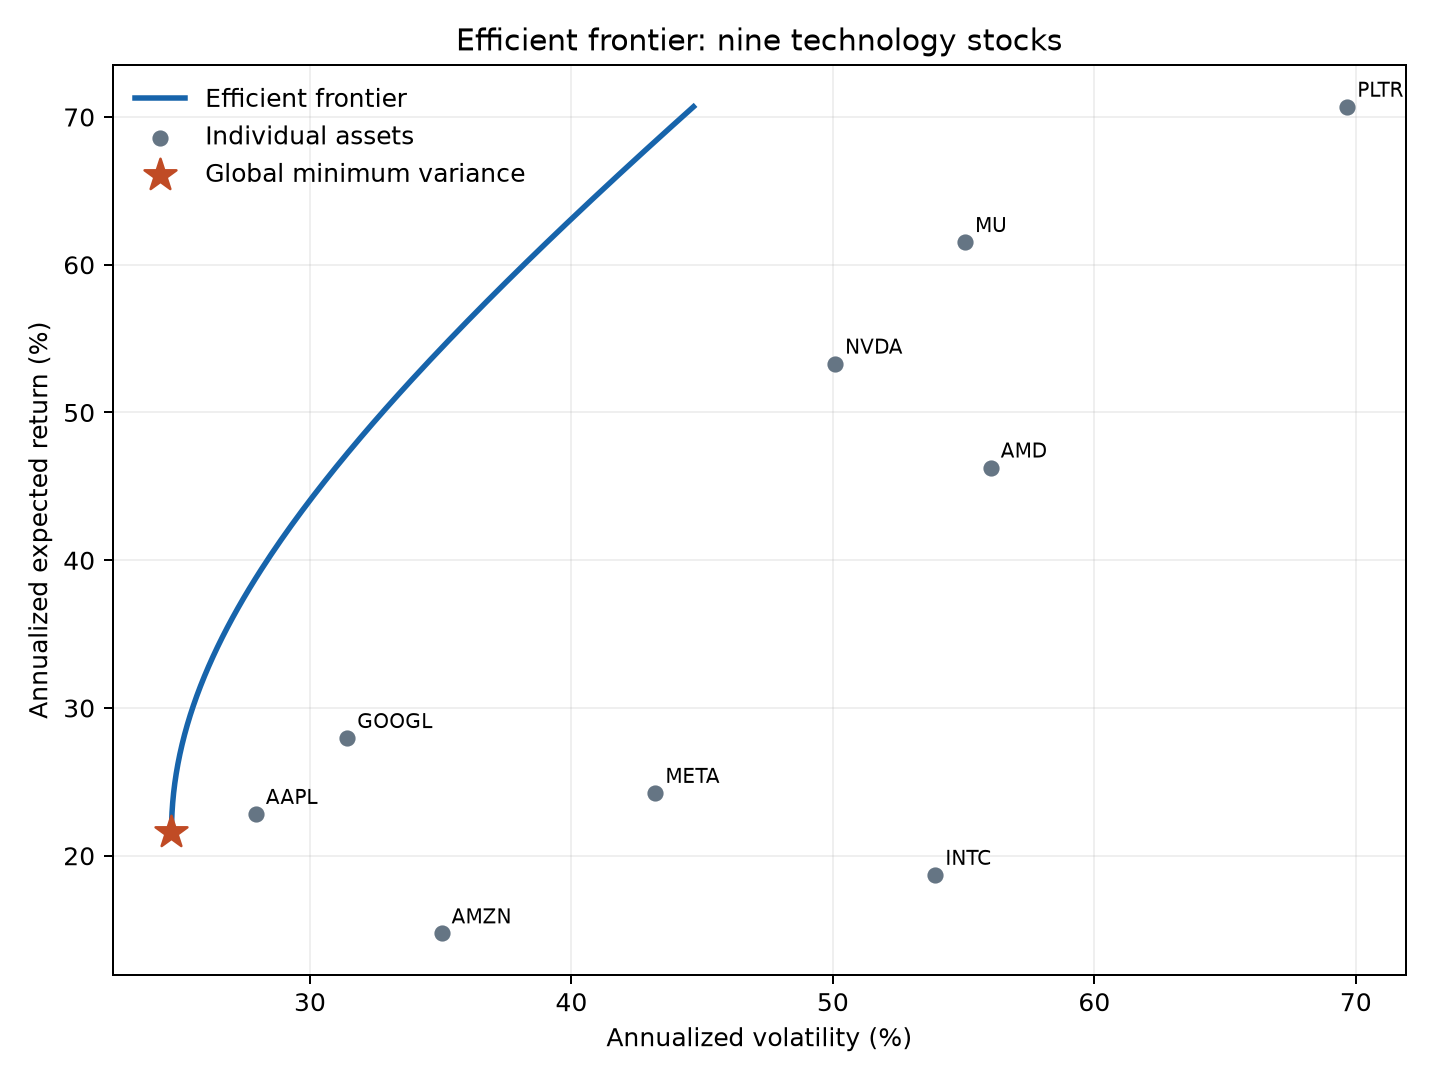
\includegraphics[width=0.9\linewidth]{real_efficient_frontier.png}
\end{center}
From the graph, we can see that as we increase our expected return,
we also have to take on more risk. The star represents the portfolio
with the lowest risk. The individual stocks are also plotted to show
how combining different stocks can help reduce portfolio risk.
\end{enumerate}

\section*{Verification Table}
\small
\begin{longtable}{@{}>{\raggedright\arraybackslash}p{2.4cm}
>{\raggedright\arraybackslash}p{2.1cm}
>{\raggedright\arraybackslash}p{3.4cm}
>{\raggedright\arraybackslash}p{4.0cm}l@{}}
\toprule
Data & Quantity & Compared with & Difference & Pass?\\
\midrule
\endfirsthead
\toprule
Data & Quantity & Compared with & Difference & Pass?\\
\midrule
\endhead
\bottomrule
\endfoot
Small example & $\w^*$ & exact scalar solution & $0$ & Yes\\
Small example & $\w^*$ & NumPy solve & $0$ & Yes\\
Small example & budget & $1$ & $0$ & Yes\\
Small example & stationarity & zero vector & $0$ & Yes\\
Sim. (2000) & $\hat\bmu$ & NumPy mean & $1.80\times10^{-16}$ & Yes\\
Sim. (2000) & $\hat\Sigma$ & NumPy covariance & $1.39\times10^{-17}$ & Yes\\
Sim. (2000) & $\hat\w$ & NumPy solve & $0$ & Yes\\
Sim. (2000) & $\w(r)$ & NumPy KKT solve & $2.22\times10^{-15}$ & Yes\\
Sim. (2000) & budget & $1$ & $0$ & Yes\\
Sim. (2000) & $\hat\bmu$ & true $\bmu$ & max standardized error $0.74$ SE & Yes\\
Sim. (2000) & $\hat\w$ & true $\w^*$ & $\|\cdot\|_2=0.0168$ & Yes\\
Sim. (50--5000) & $\hat\w$ & true $\w^*$ & largest error/SE $1.16$ & Yes\\
Sim. (60) & $\hat\w$ & true $\w^*$ & $\|\cdot\|_2=0.1530$ (9.1 times larger) & Yes (stress)\\
Duplicate asset & $\hat\Sigma$ & expected singularity & $\lambda_{\min}=-2.61\times10^{-18}$ & Yes (stress)\\
Real data & $\hat\bmu$ & NumPy mean (daily) & $8.67\times10^{-19}$ & Yes\\
Real data & $\hat\Sigma$ & NumPy covariance (daily) & $2.17\times10^{-19}$ & Yes\\
Real data & $\hat\bmu_{\rm ann}$ & NumPy mean (annual) & $2.22\times10^{-16}$ & Yes\\
Real data & $\hat\Sigma_{\rm ann}$ & NumPy covariance (annual) & $5.55\times10^{-17}$ & Yes\\
Real data & $\w^*$ & NumPy solve & $3.33\times10^{-16}$ & Yes\\
Real data & budget & $1$ & $4.44\times10^{-16}$ & Yes\\
Real data & $\w(r)$ & NumPy KKT solve & $6.11\times10^{-16}$ & Yes\\
Real data & target return & $r$ & $5.55\times10^{-17}$ & Yes\\
Real data & $\sigma^2(r)$ & direct quadratic form & $8.33\times10^{-17}$ & Yes\\
\end{longtable}
\normalsize
\end{document}
